% Свежая версия шаблона здесь <https://www.overleaf.com/read/sqvxbnhgxxdm>
\documentclass[14pt,a4paper,report]{ncc}
\usepackage[a4paper, mag=1000, left=2.5cm, right=1cm, top=2cm, bottom=2cm, headsep=0.7cm, footskip=1cm]{geometry}
\usepackage[utf8]{inputenc}
\usepackage[english,russian]{babel}
\usepackage{indentfirst}
\usepackage[dvipsnames]{xcolor}
\usepackage[colorlinks]{hyperref}
\usepackage{listings} 
\usepackage{caption}
\usepackage{amssymb}
\usepackage{tcolorbox}
\DeclareCaptionFont{white}{\color{white}} %% это сделает текст заголовка белым
%% код ниже нарисует серую рамочку вокруг заголовка кода.
\usepackage{color} %% это для отображения цвета в коде
\DeclareCaptionFormat{listing}{\colorbox{gray}{\parbox{\textwidth}{#1#2#3}}}
\captionsetup[lstlisting]{format=listing,labelfont=white,textfont=white}
\lstset{% Собственно настройки вида листинга
inputencoding=utf8, extendedchars=\true, keepspaces = true, % поддержка кириллицы и пробелов в комментариях
language=C++,            % выбор языка для подсветки (здесь это Pascal)
numberstyle =\tiny
basicstyle=\small\sffamily, % размер и начертание шрифта для подсветки кода
keywordstyle =\color{ForestGreen},
numbers=left,               % где поставить нумерацию строк (слева\справа)
numberstyle=\tiny,          % размер шрифта для номеров строк
stepnumber=1,               % размер шага между двумя номерами строк
numbersep=5pt,              % как далеко отстоят номера строк от подсвечиваемого кода
backgroundcolor=\color{white}, % цвет фона подсветки - используем \usepackage{color}
showspaces=false,           % показывать или нет пробелы специальными отступами
showstringspaces=false,     % показывать или нет пробелы в строках
showtabs=false,             % показывать или нет табуляцию в строках
frame=single,               % рисовать рамку вокруг кода
tabsize=2,                  % размер табуляции по умолчанию равен 2 пробелам
captionpos=t,               % позиция заголовка вверху [t] или внизу [b] 
breaklines=true,            % автоматически переносить строки (да\нет)
breakatwhitespace=false,    % переносить строки только если есть пробел
escapeinside={\%*}{*)}      % если нужно добавить комментарии в коде
}

\begin{document}
% Переоформление некоторых стандартных названий
%\renewcommand{\chaptername}{Лабораторная работа}
\def\contentsname{Содержание}

% Оформление титульного листа
\begin{titlepage}
\begin{center}
\textsc{ФГОУ ВО Уральский Федеральный Университет \\ имени первого Президента России Б.Н.Ельцина\\[5mm]
Физико-технологический институт\\[2mm]
Кафедра теоретической физики и прикладной математики}

\vfill

\textbf{ОТЧЁТ ПО ЛАБОРАТОРНОЙ РАБОТЕ №4\\[3mm]
«Моделирование двумерной системы частиц с дефектами типа вакансий, взаимодействующих через потенциал Леннарда Джонса»\\[6mm]
}
\end{center}

\hfill
\begin{minipage}{.5\textwidth}
Студент:\\[2mm] 
Вялова С.А.\\
группа: ФтМ-170403 \\[5mm]

Преподаватель:\\[2mm] 
д.ф.-м.н., профессор\\
Мазуренко Владимир Владимирович\\[5mm]

Консультант:\\[2mm] 
н.с.\\
Сотников Олег Михайлович\\

\end{minipage}%
\vfill
\begin{center}
\today  \\
%\theyear\, г.
 Екатеринбург.
\end{center}
\end{titlepage}

% Содержание
\tableofcontents
\newpage
\chapter{Моделирование атомной структуры реальных кристаллов}
\section{Цель работы}


Разработка компьютерной программы для моделирования двумерной системы частиц с дефектами типа вакансий, взаимодействующих через потенциал Леннарда-Джонс, используя метод Монте Карло, а именно алгоритм Метрополиса, а также с учетом ди-
намики решетки при использовании  алгоритма Верле.
\

В ходе выполнения работы необходимо реализовать следующие пункты:
\begin{itemize}
\item Исследовать изменение геометрии вблизи дефекта;
\item исследовать температурное поведение систем с дефектами;
\item описать изменение среднеквадратического отклонения и автокорреляци-
онной функции при переходе к системе с дефектами;
\item проанализировать изменение энергии системы в зависимости от числа
вакансий.
\end{itemize}

\

\newpage\section{Теоретическая часть }
\subsection{Потенциал Леннарда-Джонса}
%text
Потенциал Леннарда-Джонса представляет собой простую модель парного взаимодействия неполярных молекул, описывающая зависимость энергии взаимодействия двух частиц от расстояния между ними.
Потенциал был предложен Леннардом-Джонсом первоначально для исследования термодинамических свойств инертных газов. Наиболее часто используется так называемый (6-12)-потенциал Леннарда-Джонса, записанный в форме 
\
\begin{equation}
 U = 4 \cdot \varepsilon \cdot [(\sigma/r)^{12} - (\sigma/r)^{6}  ] ,
 \end{equation} 
где $\varepsilon$ - глубина потенциальной ямы, $\sigma$ - значение расстояния между частицами, при котором потенциал равен нулю. Шестая степень убывания отвечает электростатическому диполь-дипольному и дисперсионному притяжению; двенадцатая степень убывания потенциала моделирует достаточно жесткое отталкивание и выбрана из соображений математического удобства.
\
\subsection{Алгоритм Метрополиса}
Таким образом, у нас есть двумерная система частиц, которые могут смещаться случайным образом в пределах некой окружности вблизи начального положения, но так, что можно достичь состояния с любой энергией за конечное количество шагов (условие эргодичности). Для конечных температур следует ожидать, что энергия системы должна флуктуировать вокруг некоторого равновесного значения. Чтобы вычислять термодинамические величины необходимо разыгрывать состояния таким образом, чтобы система пришла к состоянию равновесия за какое-то разумное время. Для этих целей и служит Алгоритм Метрополиса. Его можно разбить на следующие шаги:

\vspace{8mm}
\begin{enumerate}
\item сгенерировать начальную конфигурацию системы $\alpha_k$;
\item выбрать $i$-ую частицу и сместить ее, сгенерировав тем самым пробное состояние системы  $\alpha_i$;
\item вычислить энергию нового состояния $E_i$;
\item если $E_k>E_i$, принять новое состояние системы;
\item если $E_i>E_k$, принять новое состояние с вероятностью:\\
$R=exp(\Delta E/kT)$;
\begin{itemize}
\item выбрать случайное число $0\le r\le 1$
\item положить состояние 
\[
\alpha_{k+1}=
\begin{cases}
\alpha_k, & \text{если $R\ge r$;} \\
\alpha_i, & \text{если $R<r$.}
\end{cases}
\]
\end{itemize}
\item вычислить нужные величины в состоянии $\alpha_{k+1}$, взять его за начальное и повторять с пункта 2 нужное количество шагов.
\end{enumerate}


%\caption{Зависимость температуры системы от шага по времени.}

\subsection{Алгоритм Верле}
%text
Для моделирования системы взаимодействующих частиц необходимо численно решить классические уравнения движения системы
\begin{equation}
m_{i}\dot{\vec{v_i}}=F_{i}(t, \vec{x_1}, ... ,  \vec{x_N}, \vec{v_1}, ... , \vec{v_N})
\end{equation}
\begin{equation}
\dot{\vec{x_i}}=\vec{v_i}.
\end{equation}
Чтобы начать моделировать двумерную систему взаимодействующих частиц, необходимо задать все координаты частиц, равномерно расположив их относительно друг друга, а также их скорости. Каждая пара частиц взаимодействует через потенциал Леннарда-Джонса.
\begin{equation}
\vec{r}_{n+1} = \vec{r}_{n} + \vec{v}_{n}\cdot{dt}
\end{equation}
\begin{equation}
\vec{v}_{n+1}=\vec{v}_{n}+\frac{1}{2} \cdot (\vec{a}_n+\vec{a}_{n+1})
\end{equation}
Ускорения определяем из потенциала Леннарда-Джонса:
\begin{equation}
\vec{F}_i= -\vec{\nabla}U(\vec{r}) = m_i \vec{a}_i
\end{equation}
Подставляя выражение для потенциала Леннарда-Джонса (1.1) в выражение для силы, действующей на каждую частицу со стороны системы, получаем ускорение i частицы:
\begin{equation}
\vec{a}_i=4  \varepsilon \cdot  \sum\limits_{i=j}^N \sum\limits_{j \neq i}^N{\frac{\vec{r}_{ij}}{m_i | \vec{r}_{ij}|^2}  [2  (\sigma/\vec{r}_{ij})^{12}-(\sigma/\vec{r}_{ij})^6]}
\end{equation}
Из полученных данных возможно вычислить кинетическую (1.8) и потенциальную (1.9) энергии системы:
\begin{equation}
E_{kinetic} = \sum\limits_{i=1}^N{\frac{m_i {\vec{v}}^2_i}{2}}
\end{equation}
\begin{equation}
E_{potential}=4 \varepsilon \sum\limits_{i=1}^N \sum\limits_{s=i+1}^N{ [(\sigma/\vec{r}_{is})^{12} - (\sigma/\vec{r}_{is})^{6}  ]}
\end{equation}
Полная энергия системы (1.10) вычисляется как сумма кинетических и потенциальных энергий всех частиц в системе.
\begin{equation}
E_{total}=E_{kinetic}+E_{potential}
\end{equation}
Важным критерием является неизменность полной энергии системы на каждом шаге.
\ 
Используемый для решение поставленной задачи вычислительный алгоритм требует нулевого суммарного импульса системы частиц.
Требование нулевого суммарного импульса системы удовлетворяется за счёт перенормировки заданных начальных скоростей следующим образом:
\begin{equation}
\vec{v}_{{i} \ new} = \vec{v}_i - {\frac{1}{N}}\sum\limits_{i=1}^N \vec{v}_i
\end{equation}
\newpage
\subsection{Описание  методов}
%text
В ходе работы необходимо исследовать треугольную решетку с дефектами типа вакансий. Для этого был видоизменен программный код для программы моделирования динамики двумерной системы частиц, взаимодействующих через потенциал Леннарда-Джонса, а также программы моделирования такой же системы частиц, но при использовании алгоритма Метрополиса.
\

Вакансия в заданной решетке задаётся путем исключения одной или нескольких частиц из рассмотрения. Число вакансий, а также расположение их выбирается программой произвольным образом: генерируется случайное число $n_{deleted}$ от $[1, \frac{n}{4}]$ ($n$ - число частиц в системе), задающее количество вакансий, а также массив $ i_{deleted}$ размерностью $n_{deleted}$, элементы которого также представляют из себя набор произвольных чисел, выбранных в промежутке от $[1, n]$. Число частиц в системе, соответственно, уменьшается на число вакансий, а массив координат частиц смещается, из него исключаются все элементы, соответствующие вакансиям.
\
После чего запускается либо динамика частиц при использовании алгорима Верле, либо квазидинамика, реализованная при использовании алгоритма Метрополиса.

Пусть $L_x$ - ширина треугольной решетки, $n_c$ - число частиц в каждой строке или столбце. Столбцы треугольной решетки отстоят друг от друга на $a={L_x}/{n_c}$, а каждую строку разделяет расстояние ${\frac{\sqrt{3}}{2}} a$. В каждой строке узлы смещены на $\frac{a}{2}$ относительно предыдущей строки. Высота треугольной решетки составляет $L_y={\frac{\sqrt{3}}{2}} L_x$, а общее число частиц в системе составляет $n={n_c}^2$. 
\
Параметры для квадратной решетки подбираются исходя из требования равенства плотностей  треугольной и квадратной решеток. Таким образом, сторона квадратной решетки $L=\sqrt{L_x \cdot L_y}$.
\

Энергия решетки вычисляется через потенциал Леннарда-Джонса следующим образом:
\begin{equation}
E=4 \varepsilon \sum\limits_{i=1}^N \sum\limits_{s=i+1}^N{ [(\sigma/\vec{r}_{is})^{12} - (\sigma/\vec{r}_{is})^{6}  ]}
\end{equation}
\newpage
\subsection{Результаты моделирования квазидинамики при использовании алгоритма Метрополиса}
Система задана со следующими параметрами:
\begin{itemize}
\item Линейные размеры системы по горизонтали $L_x=7$, линейные размеры системы по вертикали $L_y=\frac{\sqrt{3}}{2}L_x$;
\item число частиц $n=81$;
\item $\sigma=0.699$;
\item температурный множитель $kT=0,00005$;
\item число шагов алгоритма Метрополиса $N=10000$;
\end{itemize}

Система в начальный момент времени представлена на рисунке \ref{ris:image1}. Решетка, как можно увидеть, содержит 6 вакансий. Через некоторое количество шагов система пришла к виду, изображенному на рисунке \ref{ris:image2}, из которого видно, как вакансия влияет на эволюцию системы в ходе моделирования: решетка вновь стремится занять наиболее выгодное положение - принять треугольную конфигурацию, соответственно, наблюдается деформация структуры вблизи дефекта. 
\begin{figure}[h!]
\center{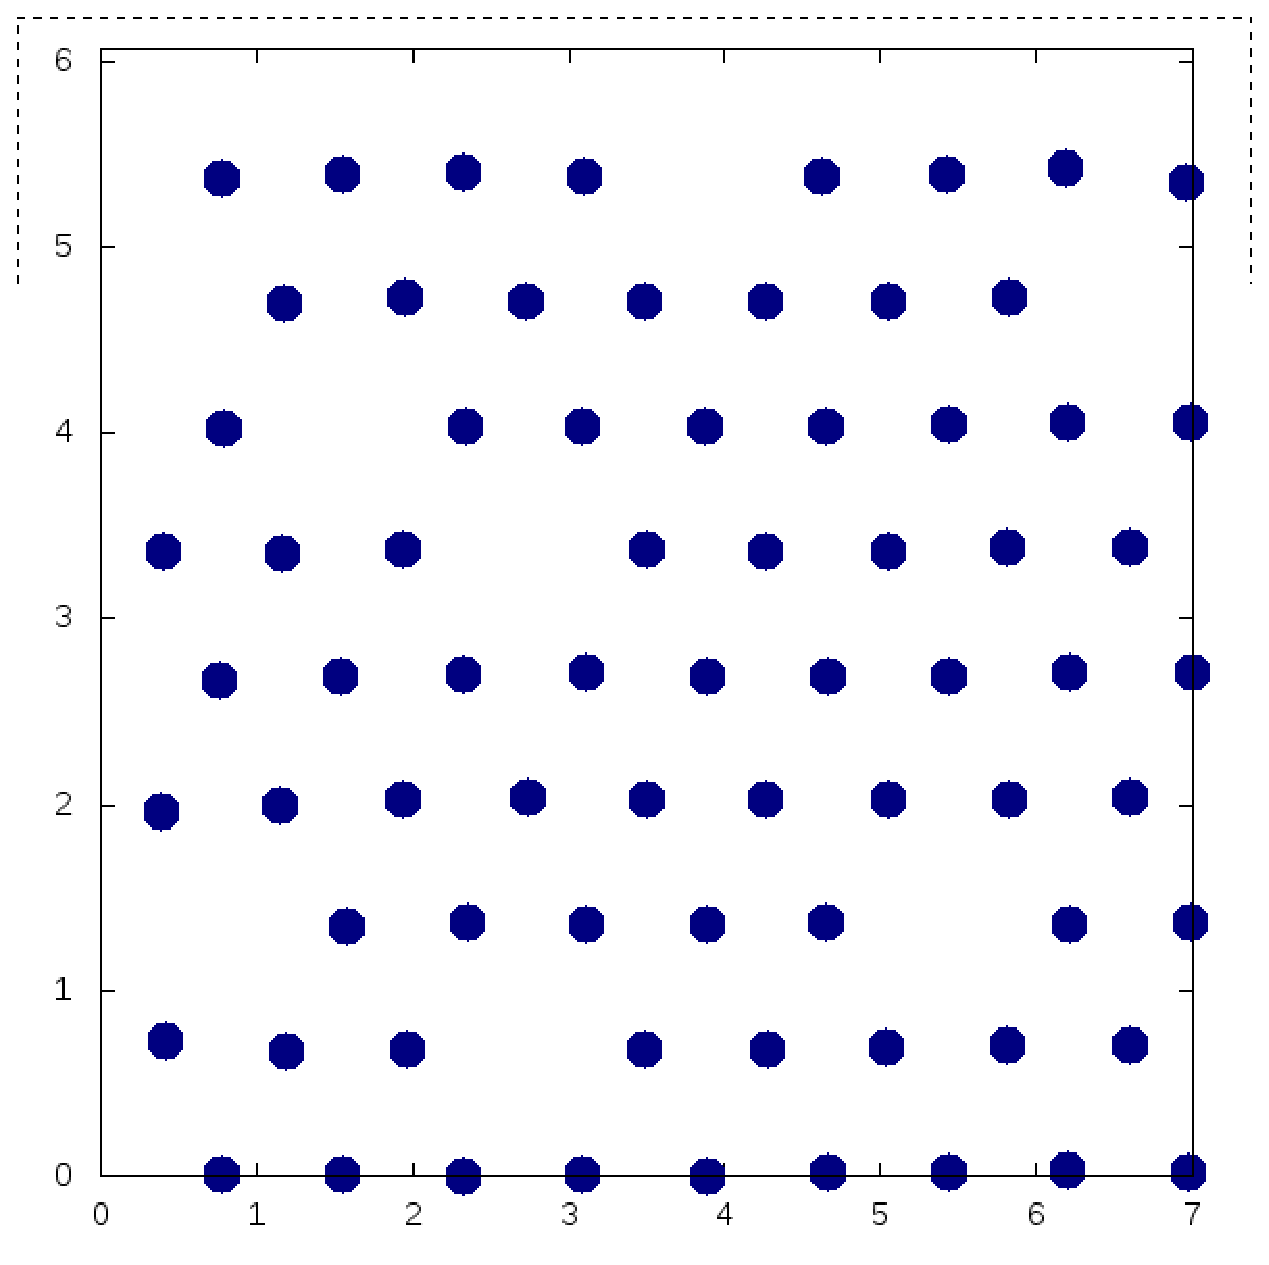
\includegraphics[width=0.65\linewidth]{pictures/system_8_vac_kT00005}}
\caption{Система с 6-ю вакансиями в начальный момент времени.}
\label{ris:image1}
\end{figure}
\begin{figure}[h!]
\center{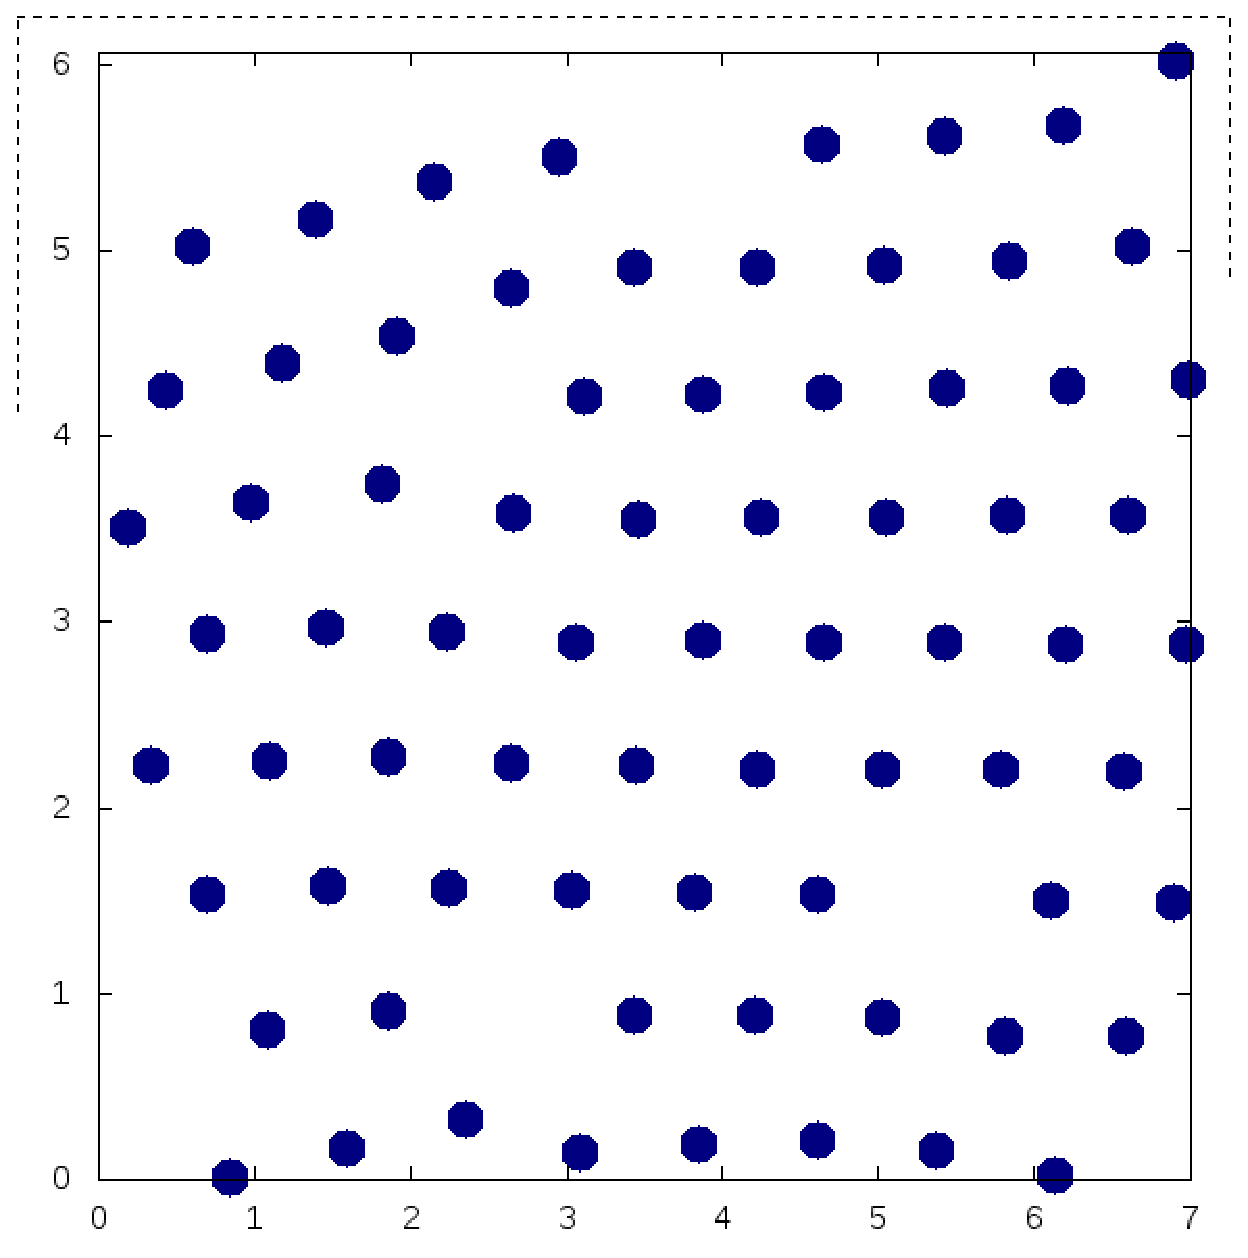
\includegraphics[width=0.65\linewidth]{pictures/system_dynamic_8_vac_kT00005}}
\caption{Система с 6-ю вакансиями в ходе моделирования.}
\label{ris:image2}
\end{figure}
Рассмотрим теперь график зависимости энергии системы от шага моделирования (\ref{ris:image3}). Система, как можно судить по данной зависимости, стремится прийти к энергетически наиболее выгодной конфигурации. 
\begin{figure}[h! ]
\center{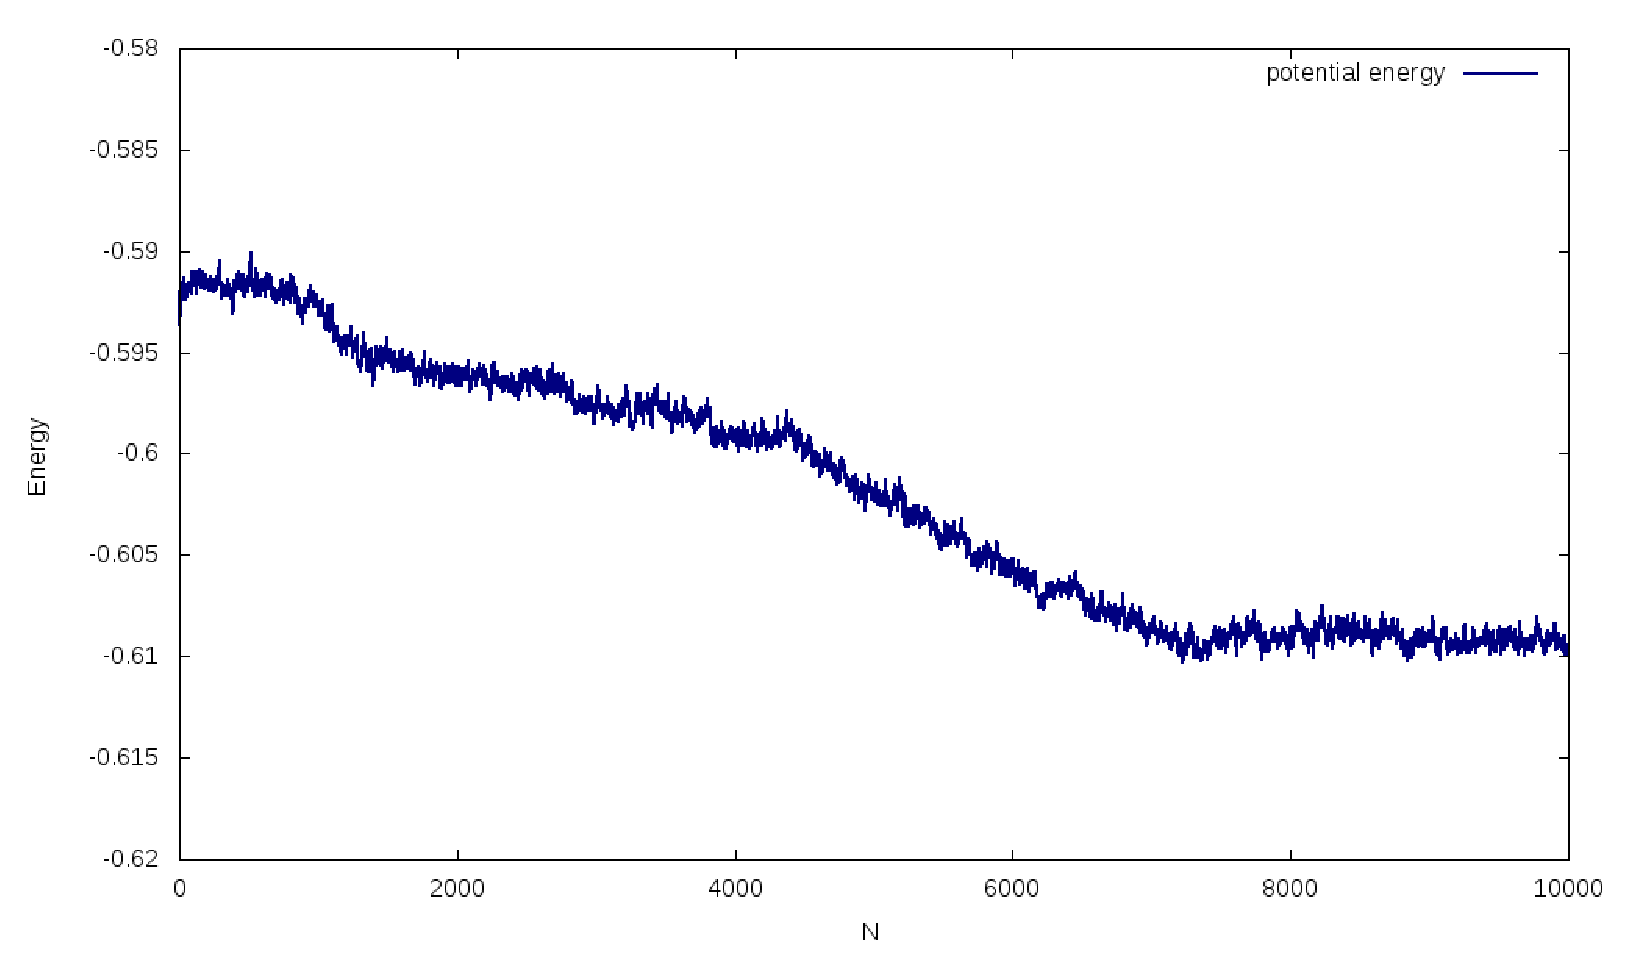
\includegraphics[width=1\linewidth]{pictures/energy_8_vac_kT00005}}
\caption{График зависимости энергии системы с 6-ю вакансиями от шага моделирования.}
\label{ris:image3}
\end{figure}
\

Более того, сразу можно сказать, что энергия системы с вакансиями выше, нежели энергия такой же системы без вакансий: расчёт основного состояния системы был проведен при помощи программы, разработанной для проведения лабораторной работы №2 (рисунок \ref{ris:image4}).
\

\begin{figure}[h!]
\center{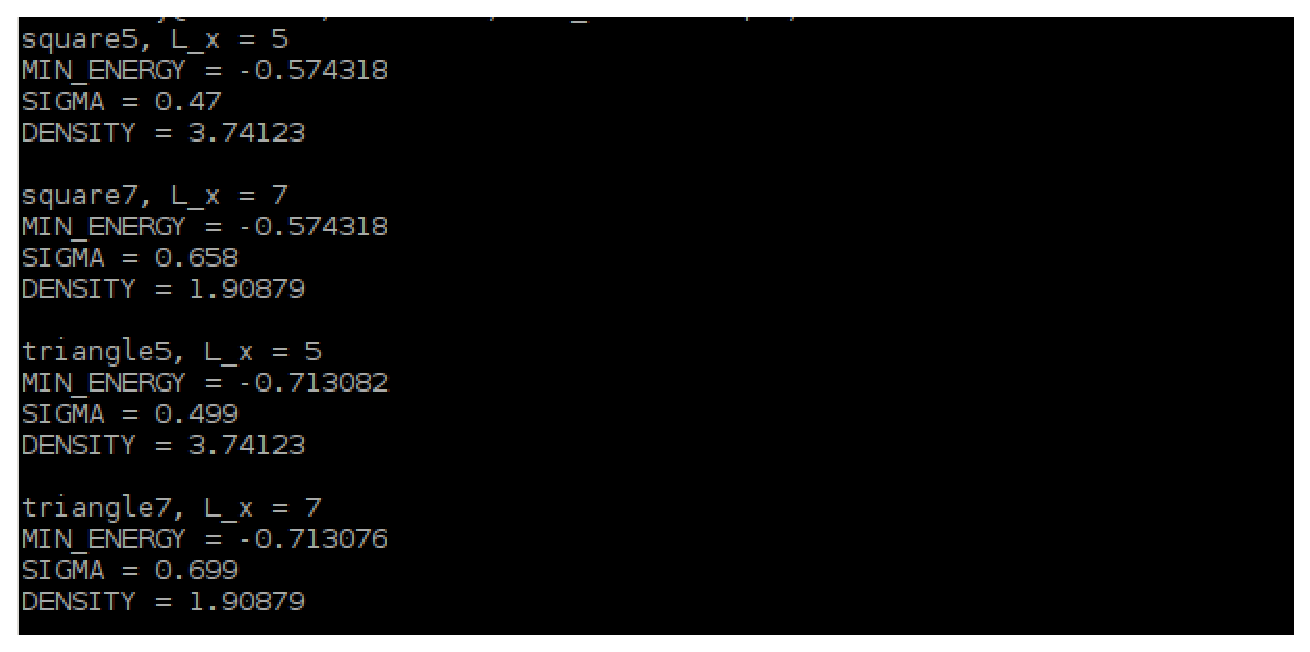
\includegraphics[width=1\linewidth]{pictures/program_lab2}}
\caption{Результат расчёта основного состояния треугольной решетки.}
\label{ris:image4}
\end{figure}
Из графика зависимости энергии системы также можно сделать вывод, что энергия равновесного состояния, к которому пришла данная система с вакансиями, выше энергии основного состояния такой же системы без вакансий.
\

График среднеквадратического отклонения частиц в ходе моделирования представлен на рисунке \ref{ris:image5}. Изменение координаты на каждом шагу мало, как можно увидеть, но это не мешает частицам прийти к равновесному положению.
\begin{figure}[h]
\center{\includegraphics[width=1\linewidth]{pictures/MSD_lie_1}}
\caption{График зависимости среднеквадратического отклонения от шага моделирования.}
\label{ris:image5}
\end{figure}
\ 

\
\newpage
Попробуем "разрушить" решетку, увеличив температурный множитель системы $kT$. Система в начальный момент времени изображена на рисунке \ref{ris:image6}, в ходе моделирования - на рисунке \ref{ris:image7}. Из графика зависимости энергии системы, изображенного на рисунке \ref{ris:image8}, очевидно, что система не является стабильной - энергия повышается, это подтверждается рисунком \ref{ris:image7}.
\begin{figure}[h]
\center{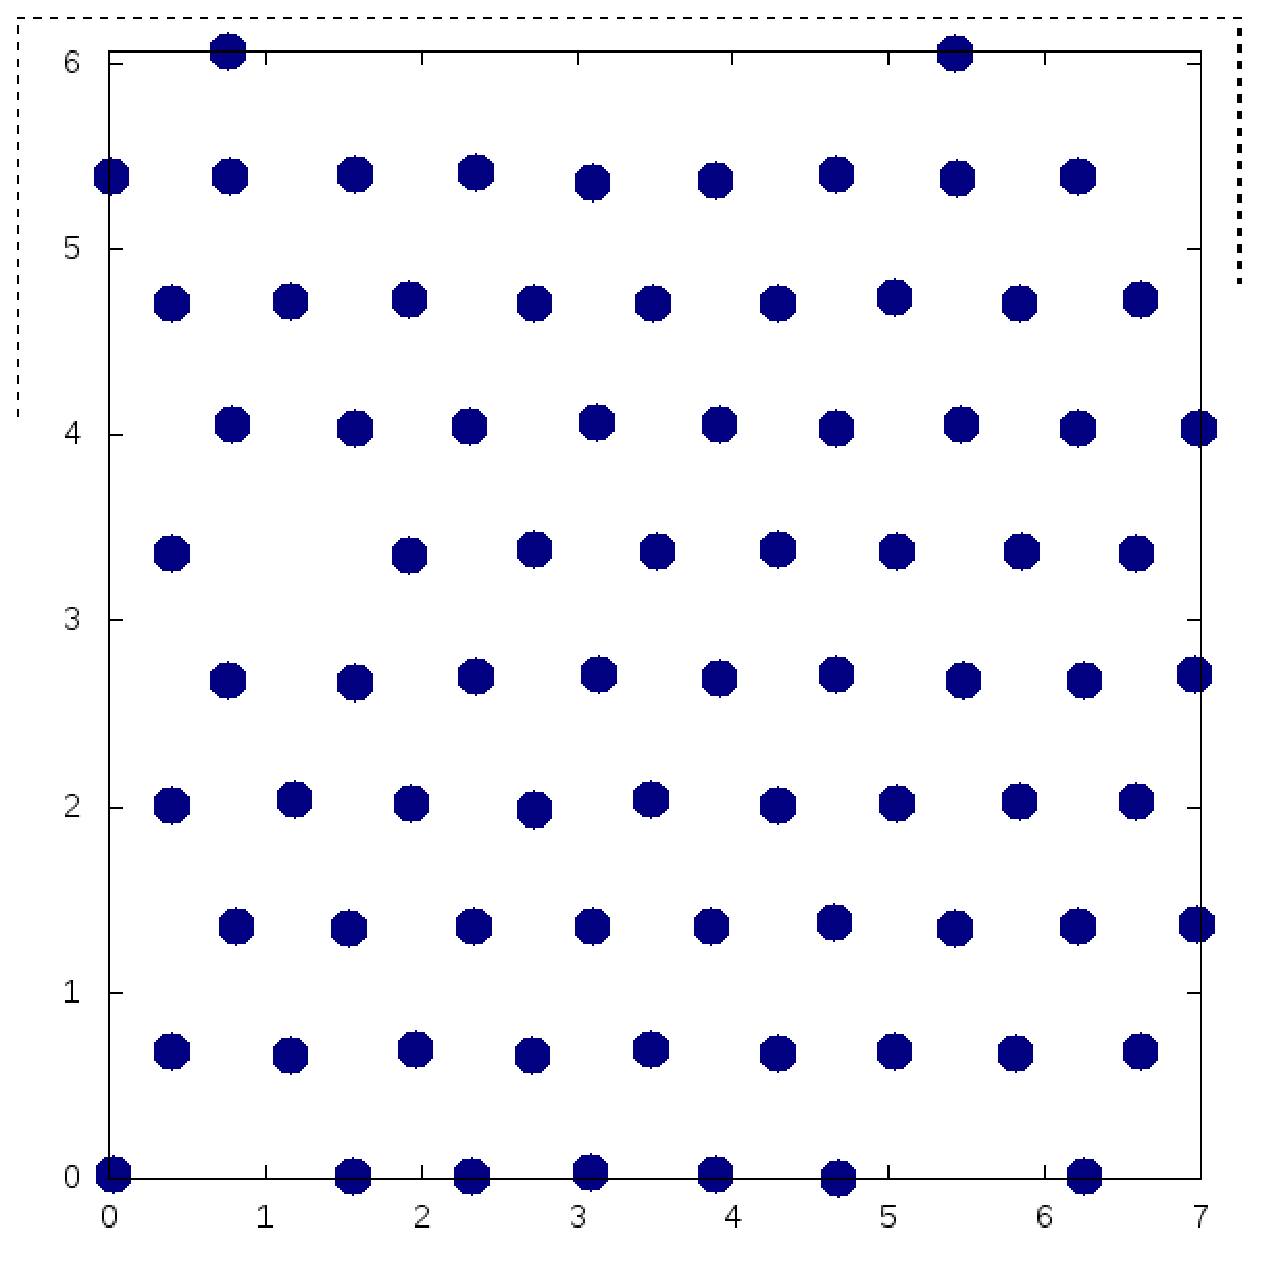
\includegraphics[width=0.6\linewidth]{pictures/system_8_vac_kT005}}
\caption{Система с 6-ю вакансиями в начальный момент времени.}
\label{ris:image6}
\end{figure}
\begin{figure}[h!]
\center{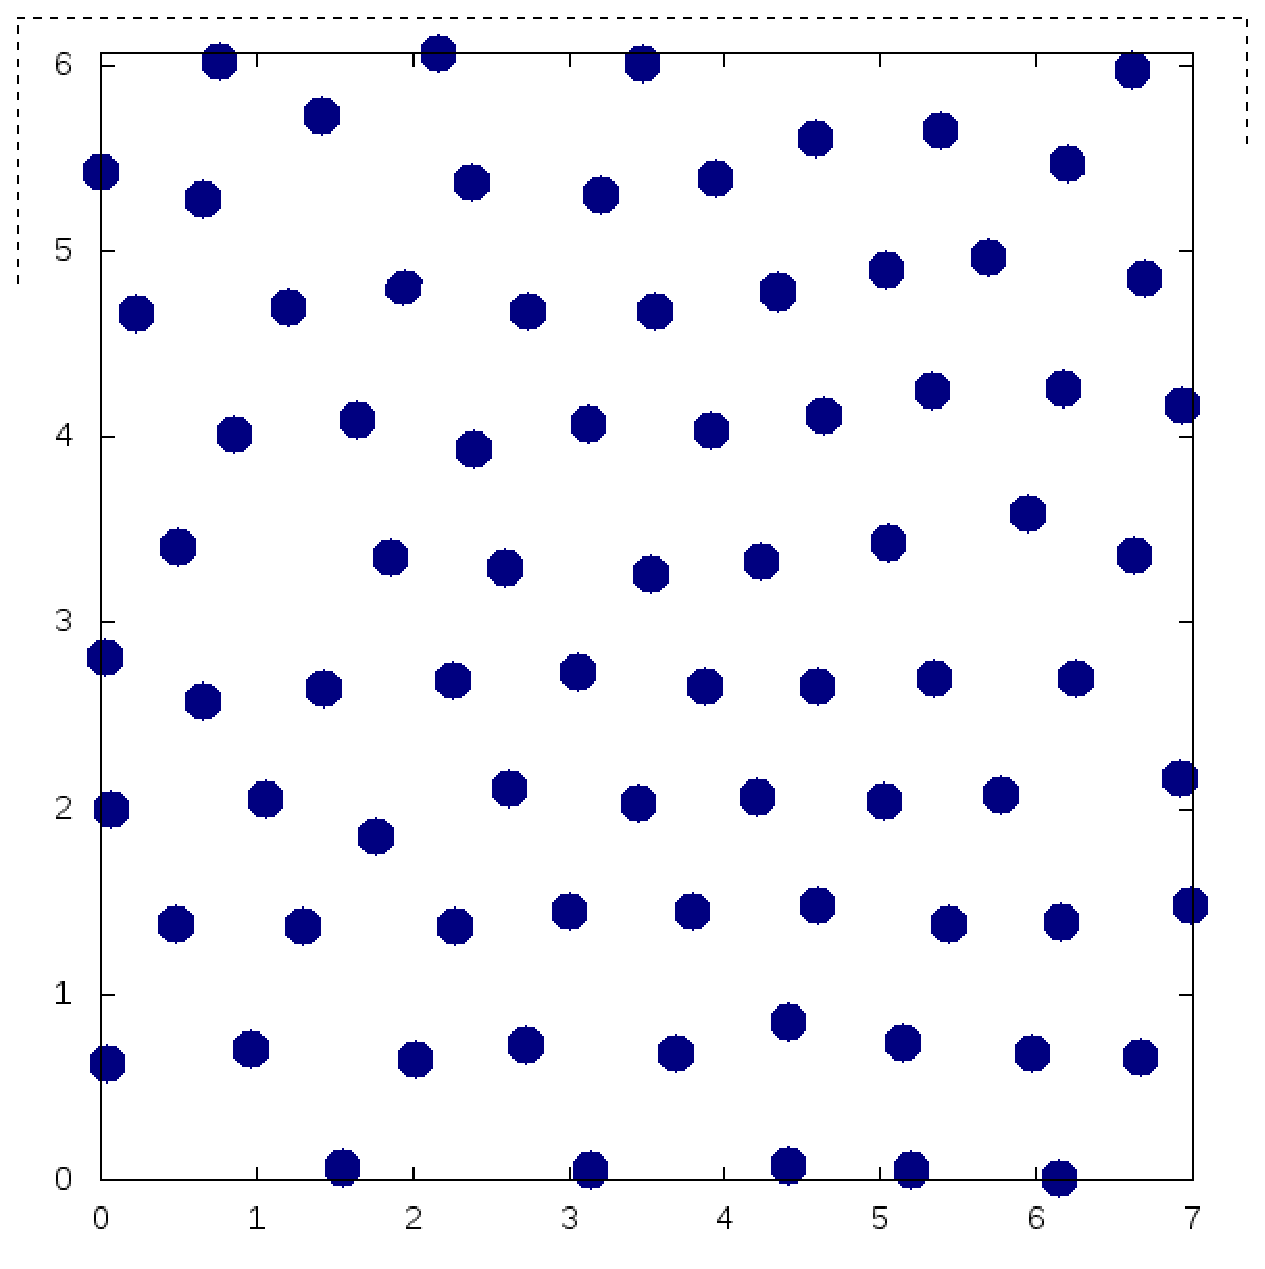
\includegraphics[width=0.6\linewidth]{pictures/system_dynamic_8_vac_kT005}}
\caption{Система с 6-ю вакансиями в ходе моделирования.}
\label{ris:image7}
\end{figure}
\begin{figure}[h!]
\center{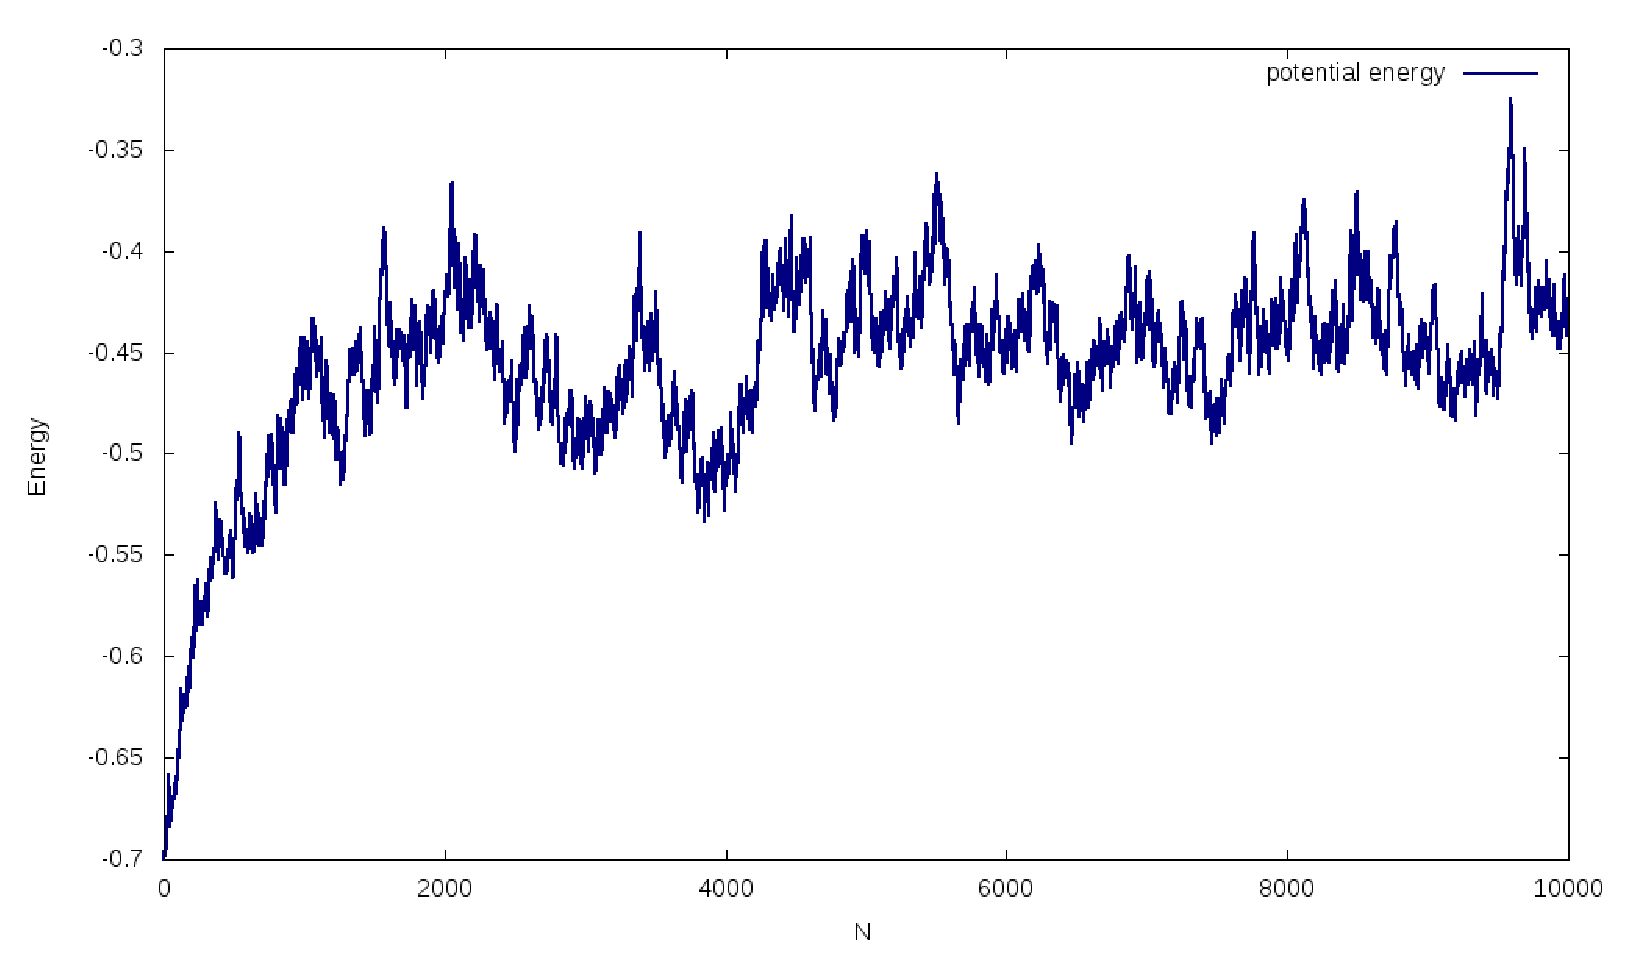
\includegraphics[width=1\linewidth]{pictures/energy_8_vac_kT005}}
\caption{График зависимости энергии системы с 6-ю вакансиями от шага моделирования.}
\label{ris:image8}
\end{figure}
Рассматривая график зависимости среднеквадратического отклонения частиц системы (рисунок \ref{ris:image9} можно сделать вывод, что частицы каждый шаг моделирования смещались на малую величину, однако это не мешало развалиться системе. 
\begin{figure}[h!]
\center{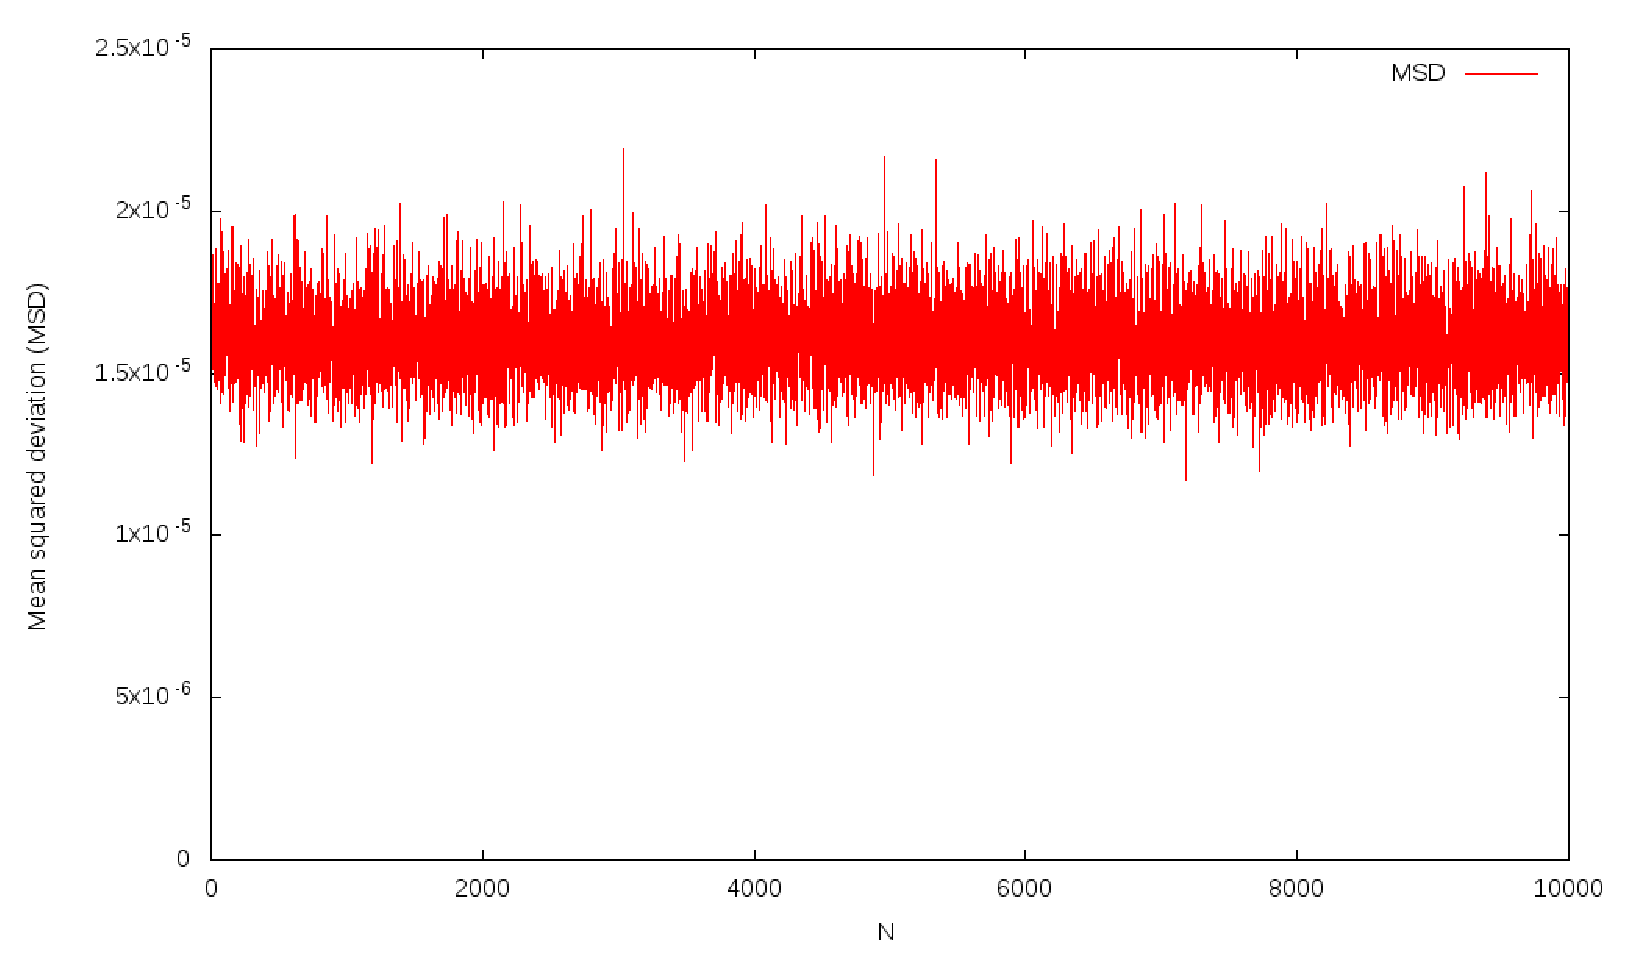
\includegraphics[width=1\linewidth]{pictures/MSD_8_vac_kT005}}
\caption{График зависимости среднеквадратического отклонения от шага моделирования.}
\label{ris:image9}
\end{figure}
\


\newpage
\subsection{Результаты моделирования квазидинамики, реализованной при использовании алгоритма Верле}
Далее рассмотрим такую же систему, но в динамике, реализованной при использовании алгоритма Верле.
\

Система задана со следующими параметрами:
\begin{itemize}
\item Линейные размеры системы по горизонтали $L_x=7$, линейные размеры системы по вертикали $L_y=\frac{\sqrt{3}}{2}L_x$;
\item число частиц $n=81$;
\item $\sigma=0.699$;
\item начальные скорости выбираются в пределе $ [-0.00001,0.00001]$;
\item число шагов алгоритма Верле  $N=300000$;
\item шаг по времени $dt=0.001$;
\end{itemize}

Первым делом рассмотрим динамику системы с малым начальным импульсом.
Начальное состояние системы представлено на рисунке \ref{ris:image10}, состояние в ходе динамики - на рисунке \ref{ris:image11}. 
\

\begin{figure}[b]
\center{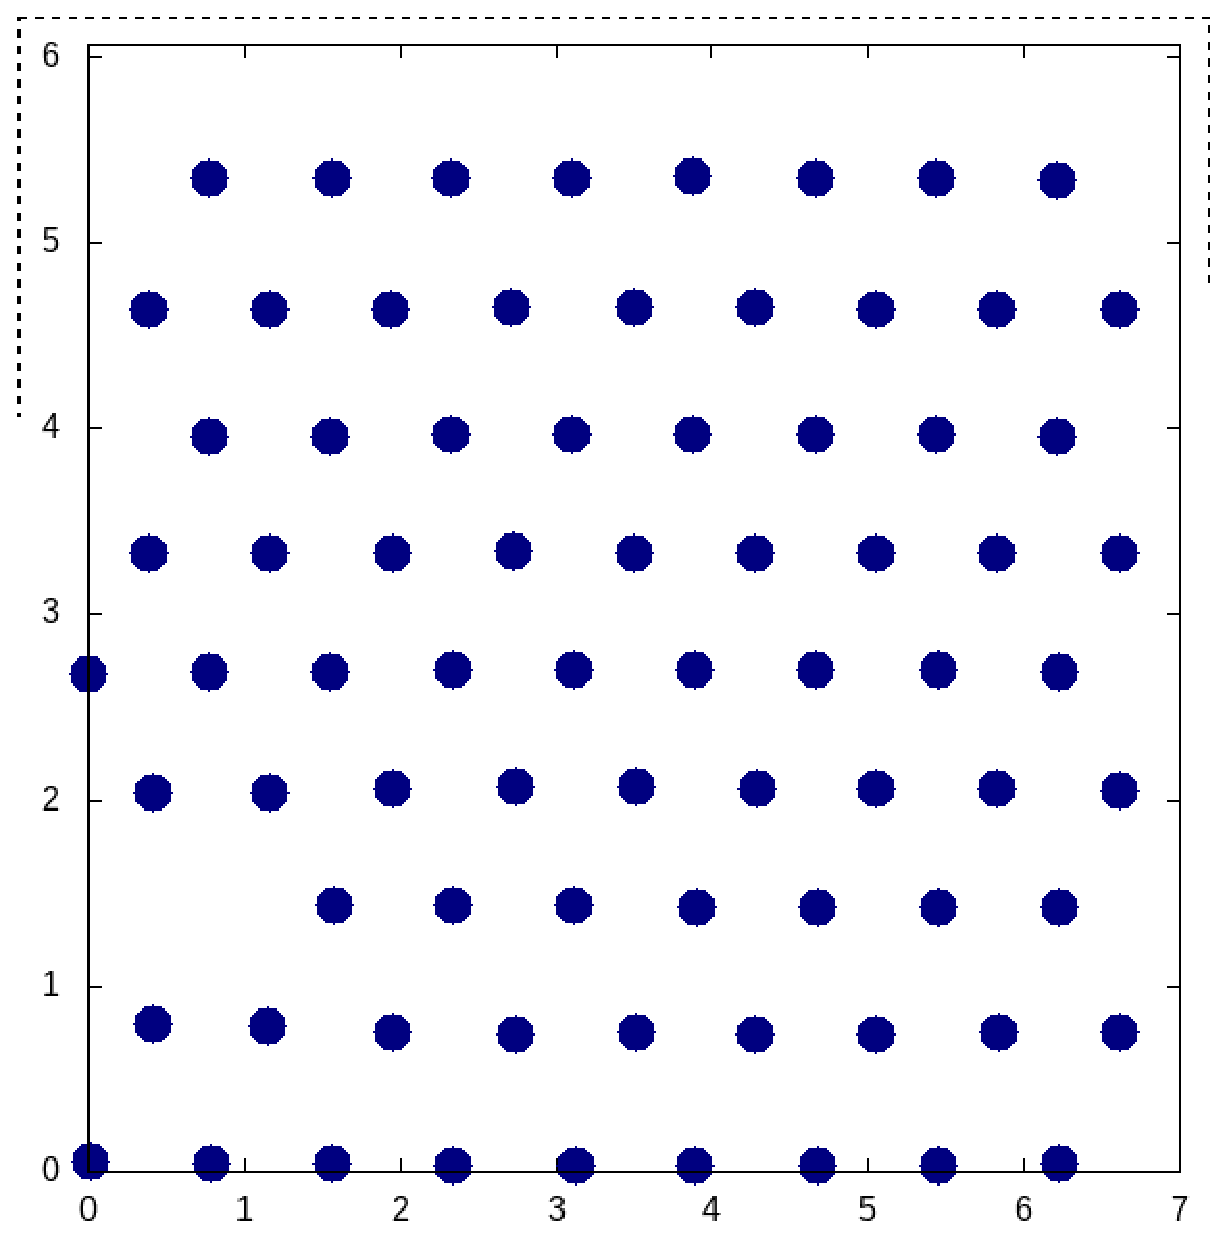
\includegraphics[width=0.7\linewidth]{pictures/system_init_dynamic}}
\caption{Система в начальный момент времени.}
\label{ris:image10}
\end{figure}
\begin{figure}[h]
\center{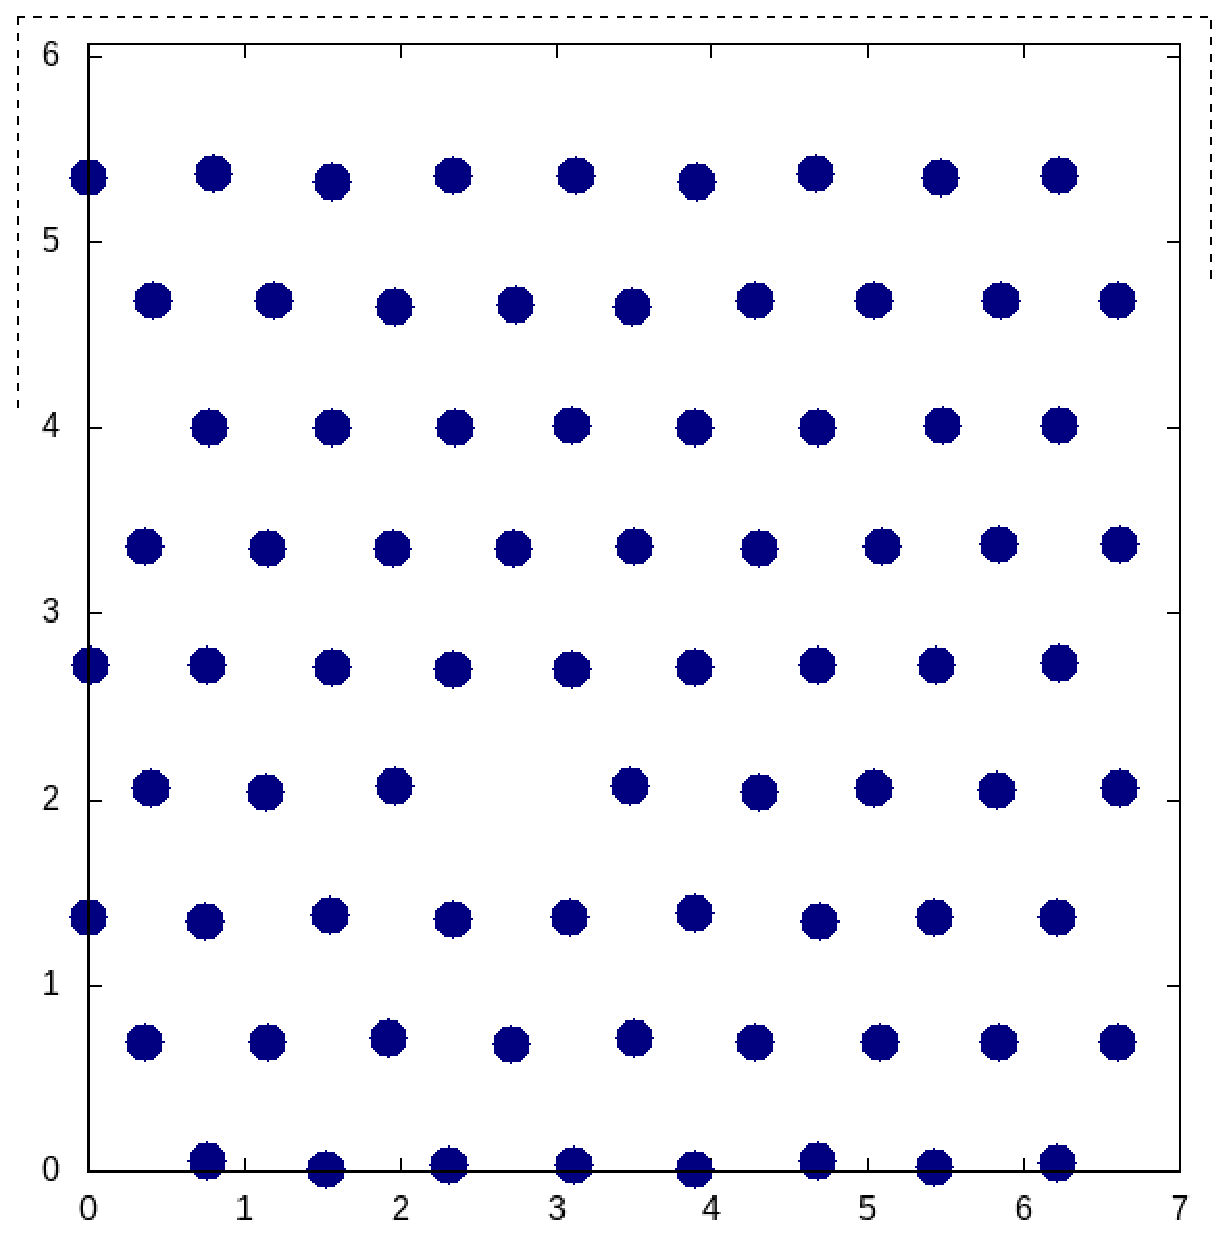
\includegraphics[width=0.7\linewidth]{pictures/system_dynamic_v00001.eps}}
\caption{Система в ходе моделирования.}
\label{ris:image11}
\end{figure}
Положение вакансии не изменилось, система стабильна при малом начальном импульсе.
\begin{figure}[h!]
\center{\includegraphics[width=1\linewidth]{pictures/energy_v00001}}
\caption{График зависимости энергии системы от шага моделирования.}
\label{ris:image12}
\end{figure}
\begin{figure}[h!]
\center{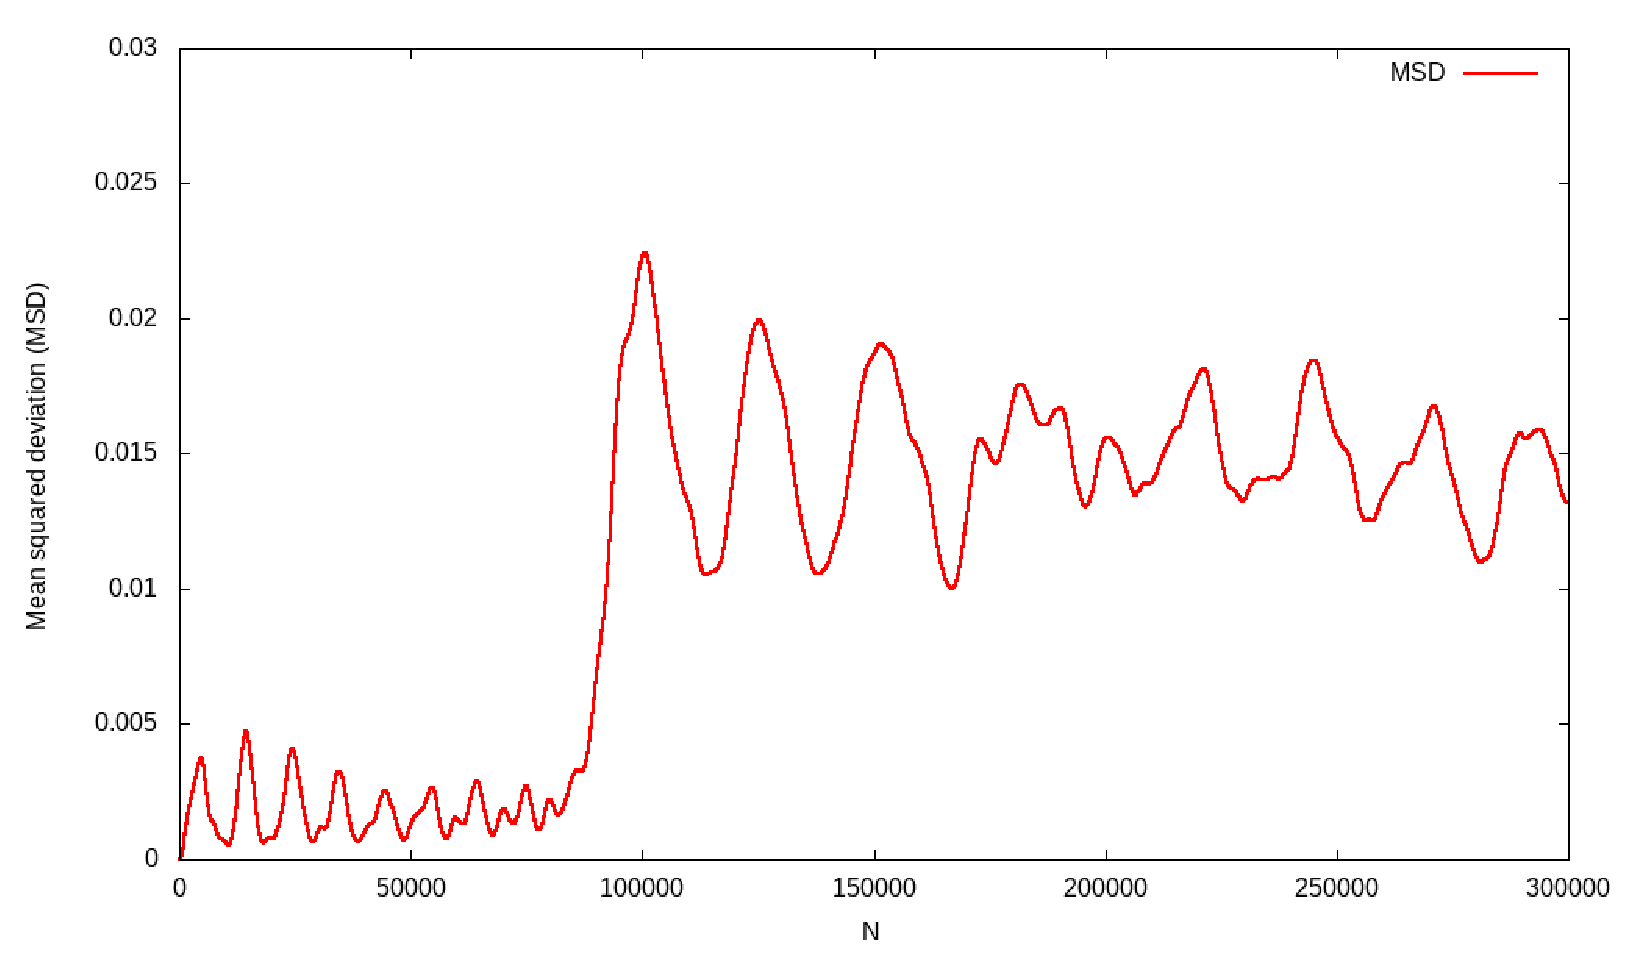
\includegraphics[width=1\linewidth]{pictures/MSD_v00001}}
\caption{График зависимости среднеквадратического отклонения от шага моделирования.}
\label{ris:image13}
\end{figure}
\begin{figure}[h!]
\center{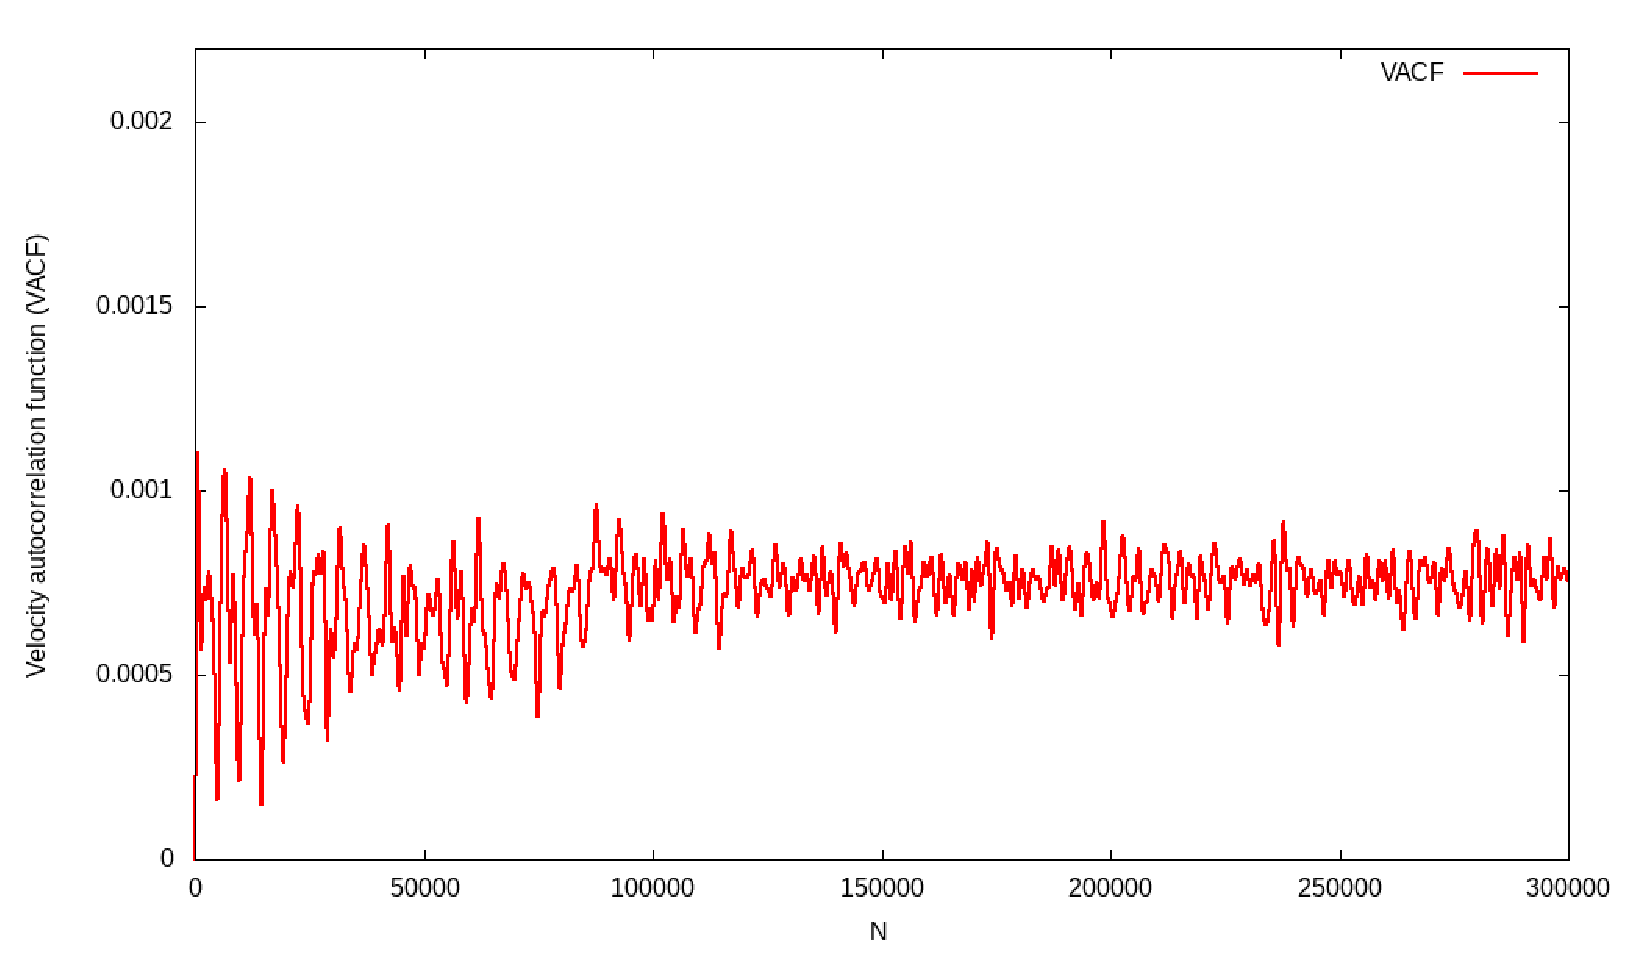
\includegraphics[width=1\linewidth]{pictures/VACF_v00001}}
\caption{График зависимости автокорреляционной функции скорости от шага моделирования.}
\label{ris:image14}
\end{figure}
\begin{figure}[h!]
\center{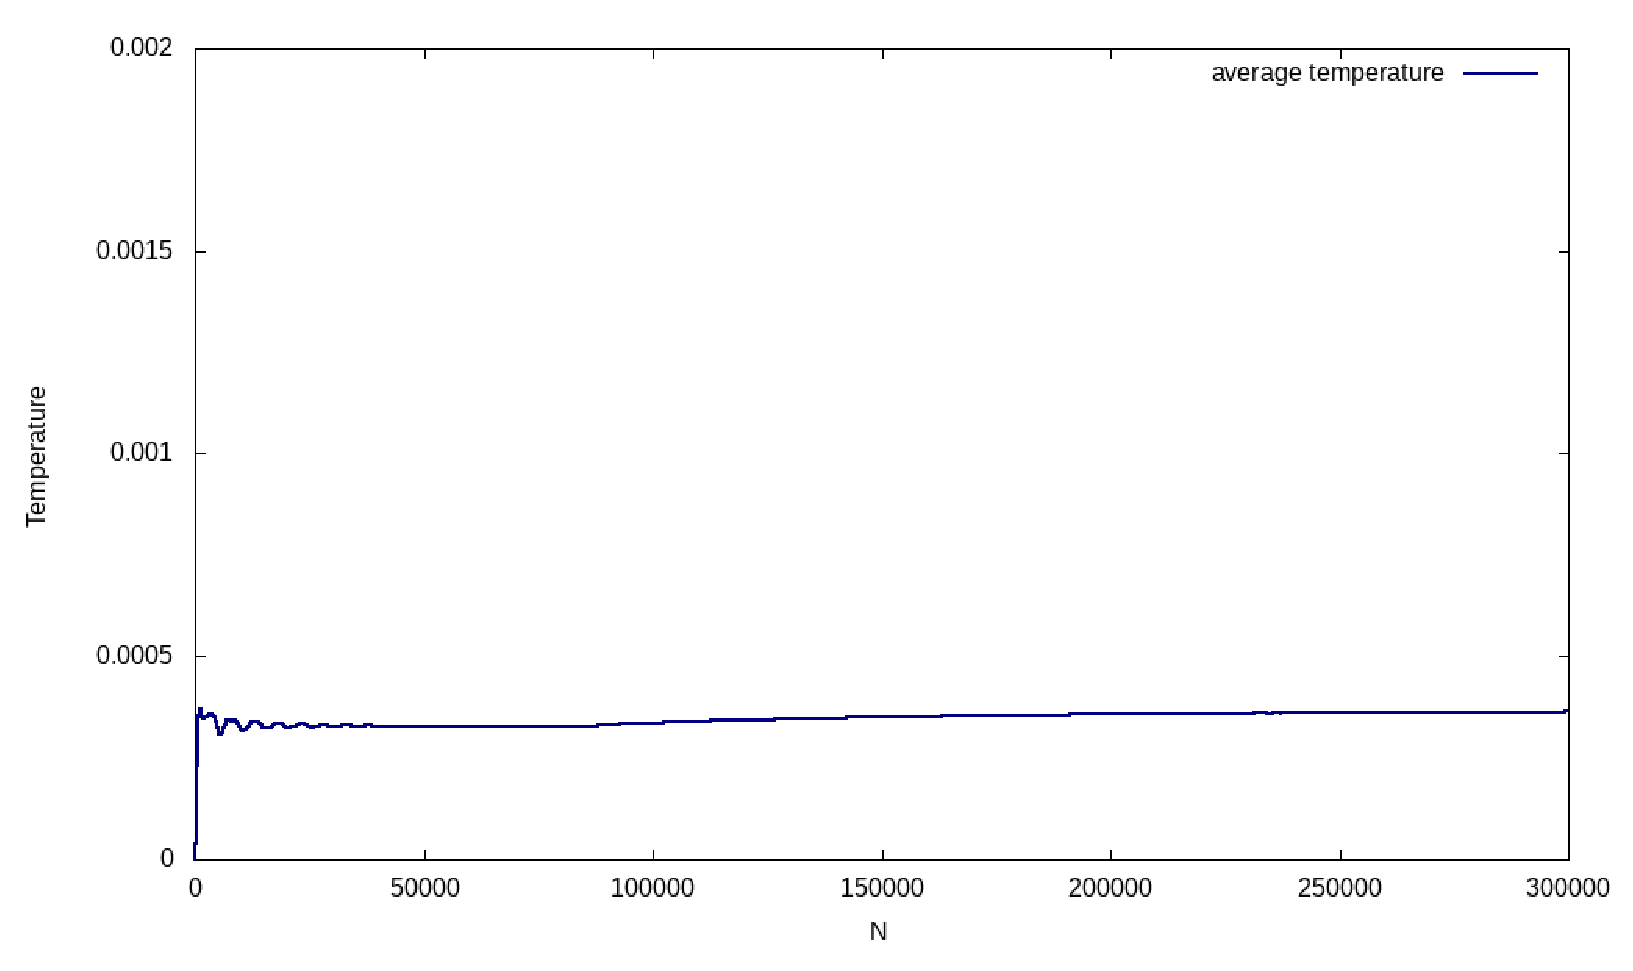
\includegraphics[width=1\linewidth]{pictures/temp_v00001}}
\caption{График зависимости температуры системы от шага моделирования.}
\label{ris:image15}
\end{figure}
График зависимости энергии системы от шага от времени, представленный на рисунке \ref{ris:image12}, указывает на то,что частицы испытывают столкновения, и изменение кинетической энергии в ходе этих столкновений по мере увеличения шага моделирования уменьшается, соответственно, система стабилизируется в некотором состоянии с чуть смещенной геометрией, обусловленной наличией вакансии. График потенциальной энергии системы хорошо согласуется с результатом, полученным в ходе моделирования подобной системы при помощи алгоритма Метрополиса. 
\

Графики зависимостисреднеквадратического отклонения и автокорреляционной функции скорости от шага моделирования представлены, соответственно, на рисунках \ref{ris:image13} и \ref{ris:image14}
Средняя температура системы, представленная на рисунке \ref{ris:image15} несколько увеличивается в ходе моделирования. Это связано с наличием вакансии в системе.
\

\newpage
Рассмотрим эту же систему, но с большим начальным импульсом, а именно - скорости частиц в начальный момент времени выбираются произвольно в промежутке $[-0,01, 0,01]$. Система в начальный момент времени выглядит как \ref{ris:image16.1}.
Cостояние в ходе динамики - на рисунке \ref{ris:image16}. 
\begin{figure}[h!]
\center{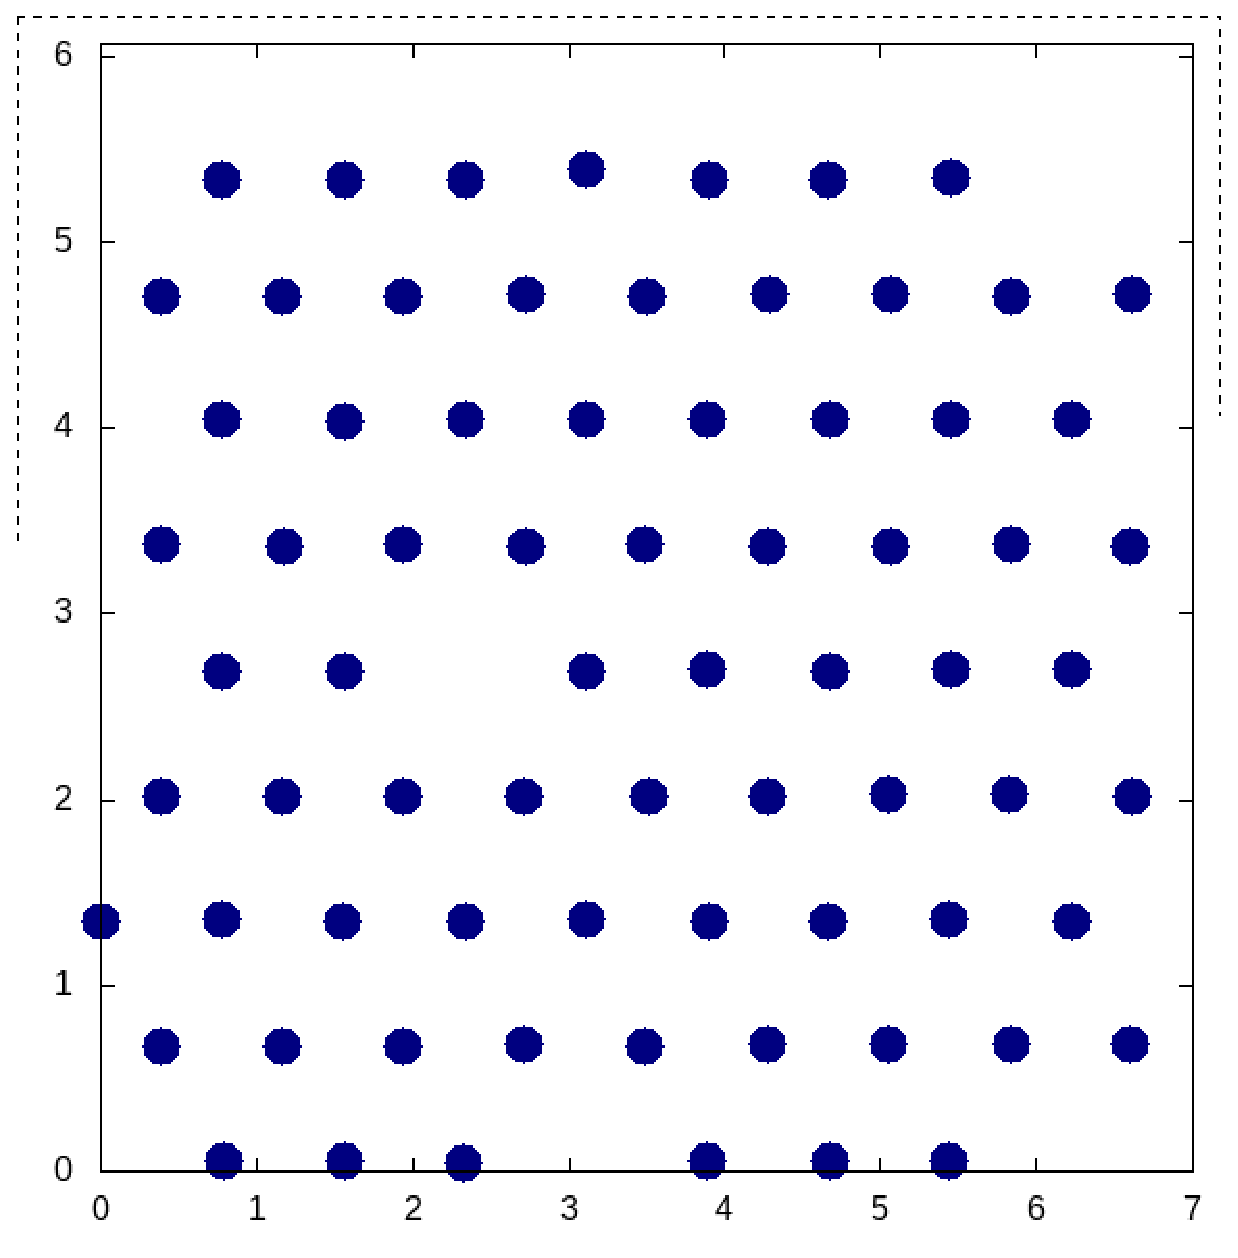
\includegraphics[width=0.6\linewidth]{pictures/system_init_v001}}
\caption{Система в начальный момент времени.}
\label{ris:image16.1}
\end{figure}
\begin{figure}[h!]
\center{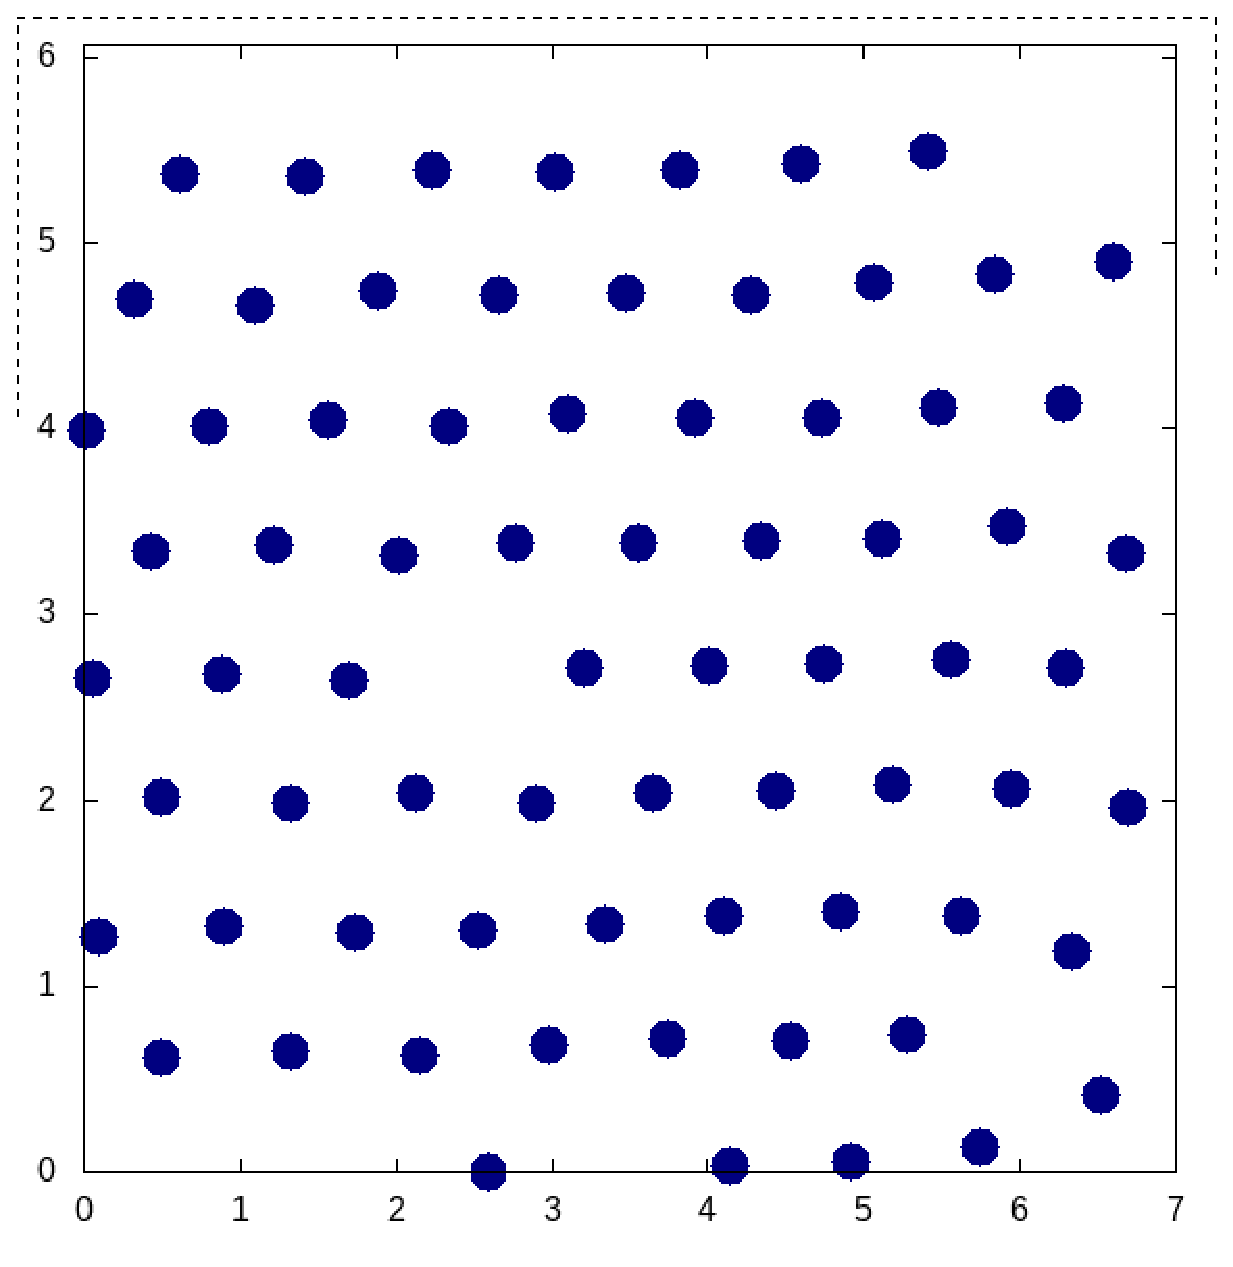
\includegraphics[width=0.61\linewidth]{pictures/system_dynamic_v001.eps}}
\caption{Система в ходе моделирования.}
\label{ris:image16}
\end{figure}
Положение вакансии в ходе моделирования постоянно изменяется. Решетка не является стабильной.
\begin{figure}[h!]
\center{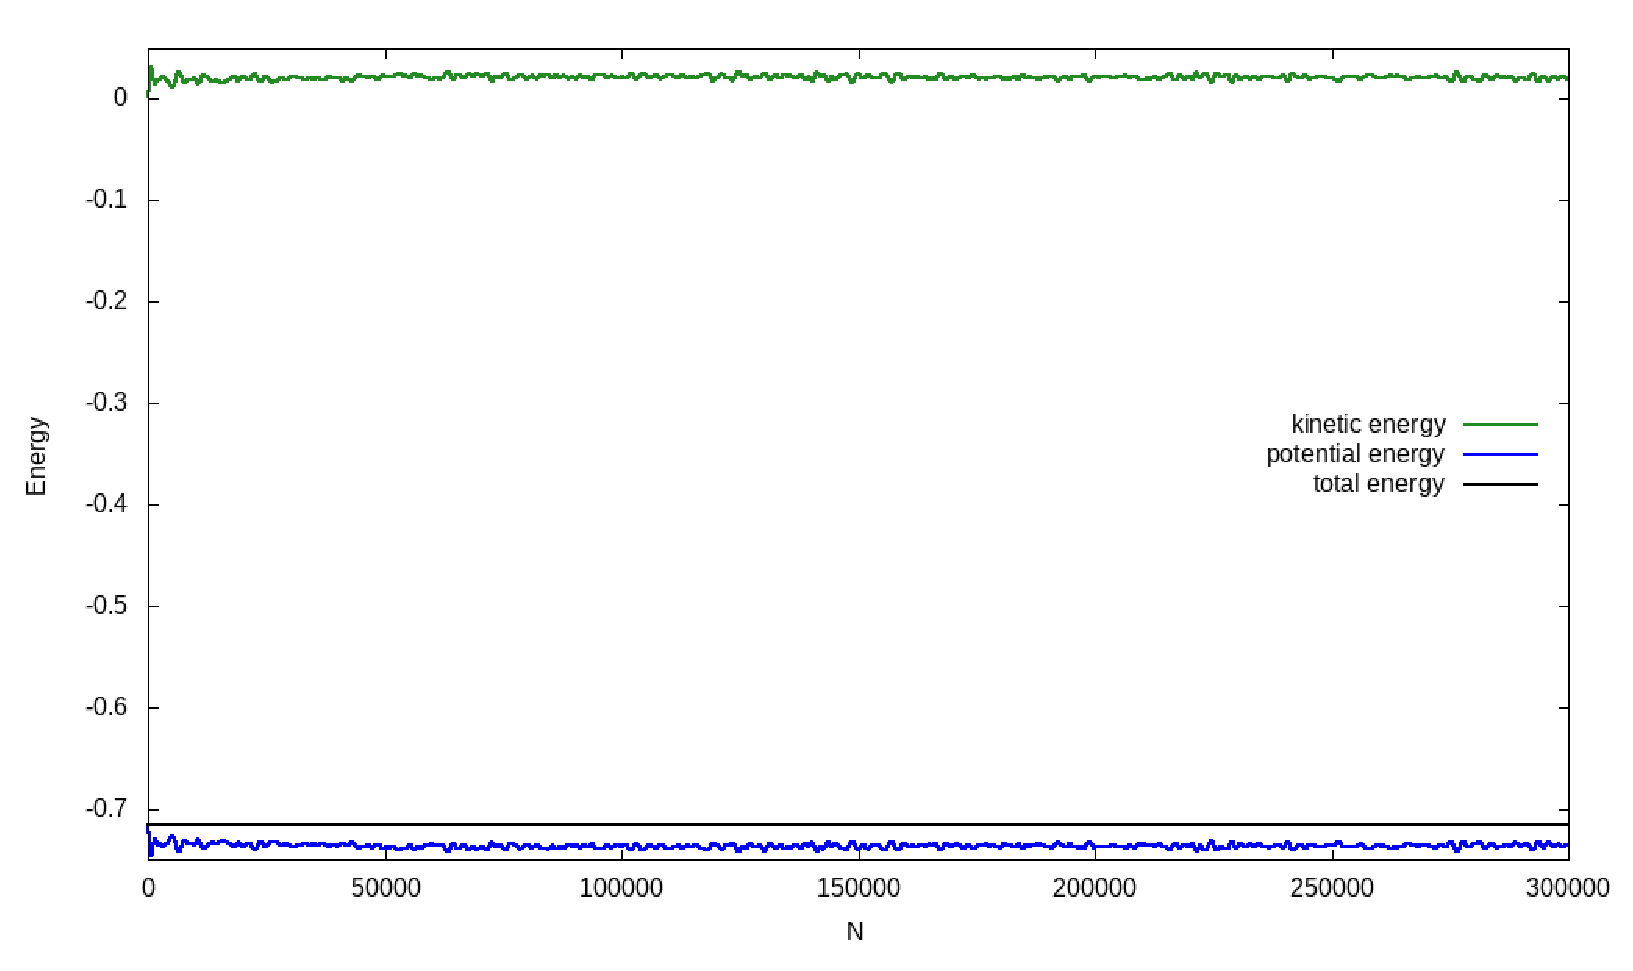
\includegraphics[width=1\linewidth]{pictures/energy_v001}}
\caption{График зависимости энергии системы от шага моделирования.}
\label{ris:image17}
\end{figure}
\begin{figure}[h!]
\center{\includegraphics[width=1\linewidth]{pictures/MSD_v001}}
\caption{График зависимости среднеквадратического отклонения от шага моделирования.}
\label{ris:image18}
\end{figure}
\begin{figure}[h!]
\center{\includegraphics[width=1\linewidth]{pictures/VACF_v001}}
\caption{График зависимости автокорреляционной функции скорости от шага моделирования.}
\label{ris:image19}
\end{figure}
\begin{figure}[h!]
\center{\includegraphics[width=1\linewidth]{pictures/temp_v001}}
\caption{График зависимости температуры системы от шага моделирования.}
\label{ris:image20}
\end{figure}
\

Из графика зависимости энергии системы, представленного на рисунке \ref{ris:image17}, можно увидеть, кинетическая энергия системы стала выше, нежели в аналогичной системе с меньшим начальным импульсом. Среднеквадратическое отклонение частиц в ходе динамики (рисунок \ref{ris:image18}) при увеличении стартового импульса системы увеличилось относительно такой же системы, у которой был стартовый импульс на два порядка меньше. График автокорреляционной функции скорости от шага моделирования представлен на рисунке \ref{ris:image19}. Температура системы в ходе моделирования медленно повышалась, что говорит о том, что решетка разваливается.
\
\newpage
\subsection{Влияние количества вакансий на энергию системы}
Исследуем, как число вакансий влияет на энергию системы. Для этого напишем простую программу, вычисляющую энергию треугольной решетки в зависимости от количества вакансий в ней.
\

График соответствующей зависимости представлен на рисунке \ref{ris:image21}, из которого очевидно, что зависимости имеет линейный характер: при увеличении числа вакансий в системе энергия системы растёт.
\begin{figure}[h!]
\center{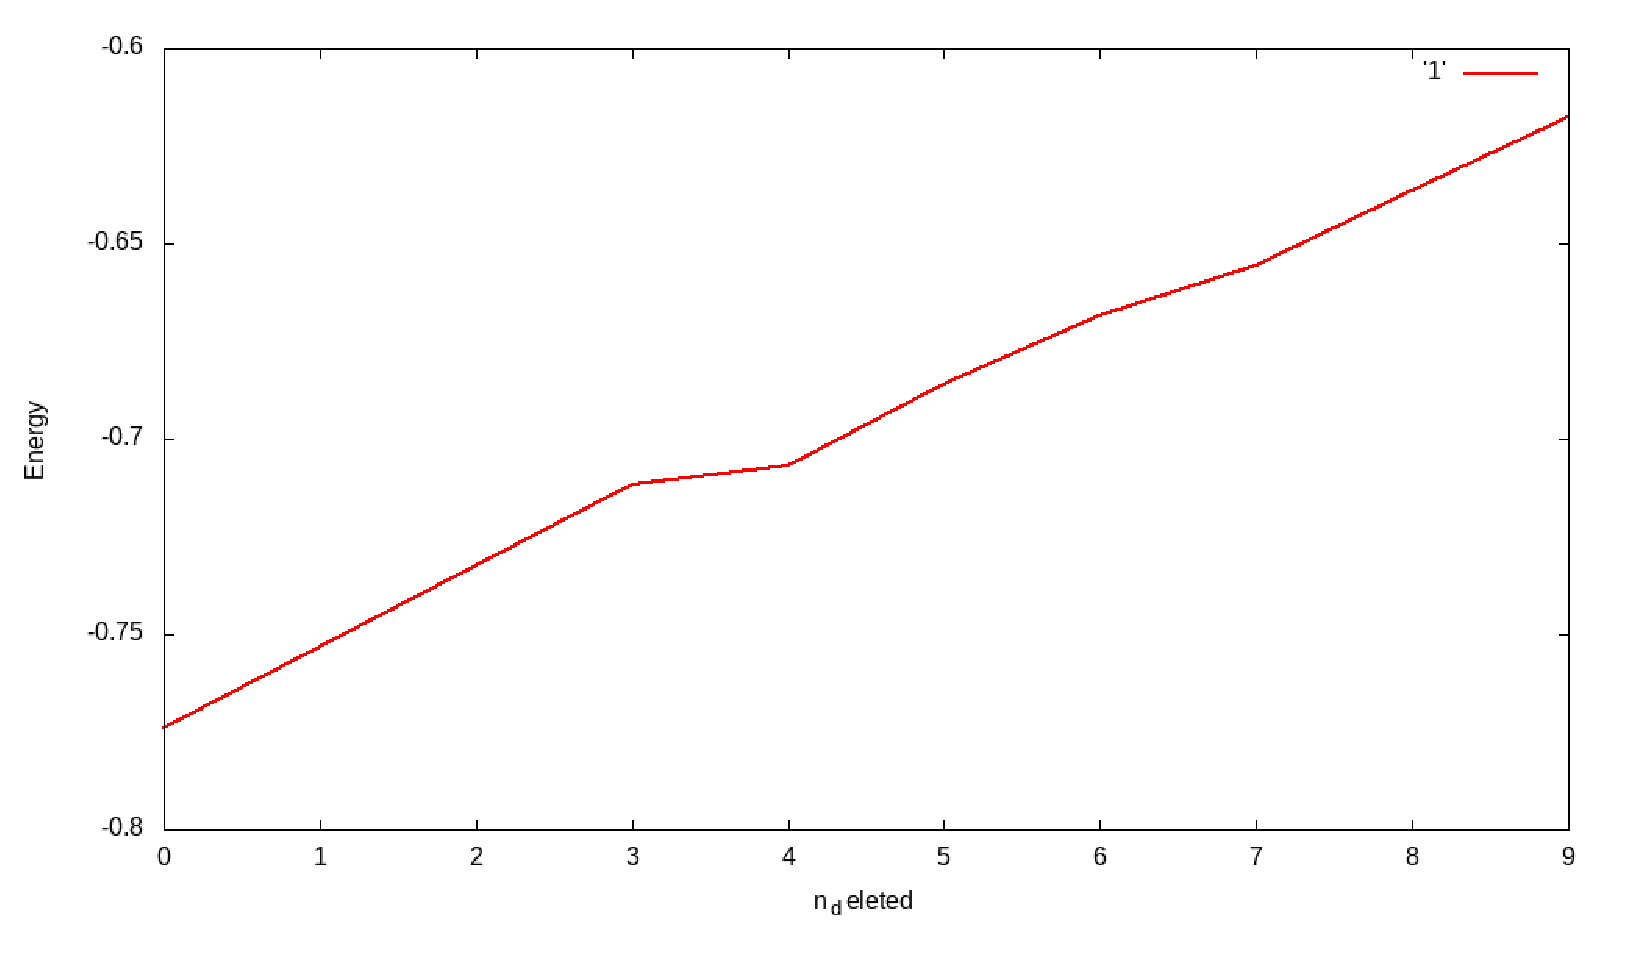
\includegraphics[width=1\linewidth]{pictures/envac}}
\caption{График зависимости энергии системы от числа вакансий.}
\label{ris:image21}
\end{figure}
\newpage
\subsection{Выводы}
В ходе данной работы было произведено моделирование систем частиц с дефектами типа вакансий. Взаимодейтствие между частицами задаётся через потенциал Леннарда-Джонса. Для моделирования систем были использованы программы, разработанные для лабораторных работ №1 и №3, в которых, соответственно, реализованы методы моделирования динамики частиц при использовании алгоритма Верле и метода Монте-Карло. Программы были дополнены возможностью исключать произвольное число произвольных частиц из рассмотрения, тем самым моделируя дефекты типа вакансий в системе. 
\

В ходе моделирования систем были исследованы графики зависимостей энергий систем от шага моделирования, и зависимости показали то, что энергия систем с дефектами выше, нежели энергия систем без дефектов, расчёты для которых были произведены в предыдущих лабораторных работах. Также было отслежено изменение геометрии системы частиц вблизи дефектов. Также, в случаях моделирования и методом Метрополиса, и методом Верле, при подборе определенной температуры системы в первом случае и подборе начального импульса - во втором, было выяснено, что вакансии свойственно изменять своё положение в решетке, и это влияет на величину среднеквадратического смещения частиц системы.
\

Также была исследована зависимость энергии системы в зависимости от количества вакансий в решетке: при росте количества дефектов в системе энергия решетки растёт.
\end{document}